\clearpage
\subsubsection{\Optimizing MSVC + \olly}
\index{\olly}

\RU{Можем попробовать этот (соптимизированный) пример в}
\EN{We can try this (optimized) example in} \olly.
\RU{Вот самая первая итерация}\EN{Here is the first iteration}:

\begin{figure}[H]
\centering
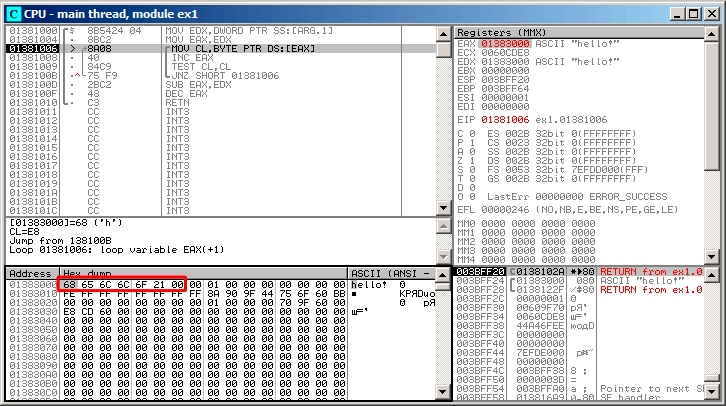
\includegraphics[scale=\FigScale]{patterns/10_strings/1_strlen/olly1.png}
\caption{\olly: \RU{начало первой итерации}\EN{first iteration start}}
\label{fig:strlen_olly_1}
\end{figure}

\RU{Видно, что \olly обнаружил цикл и, для удобства, \IT{свернул} инструкции тела цикла в скобке.}
\EN{We see that \olly found a loop and, for convenience, \IT{wrapped} its instructions in brackets.}
\RU{Нажав правой кнопкой на}\EN{By clicking the right button on} \EAX, \RU{можно выбрать}\EN{we can choose} 
\q{Follow in Dump} 
\RU{и позиция в окне памяти будет как раз там, где надо.}
\EN{and the memory window scrolls to the right place.}
\RU{Здесь мы видим в памяти строку}\EN{Here we can see the string} \q{hello!}\EN{ in memory}.
\RU{После неё имеется как минимум 1 нулевой байт, затем случайный мусор}\EN{There is at least
one zero byte after it and then random garbage}.
\RU{Если \olly видит, что в регистре содержится адрес какой-то строки, он показывает эту строку.}
\EN{If \olly sees a register with a valid address in it, that points to some string, 
it is shown as a string.}

\clearpage
\RU{Нажмем}\EN{Let's press} F8 (\stepover) \RU{столько раз, чтобы текущий адрес снова был 
в начале тела цикла}\EN{a few times, to get to the start of the body of the loop}:

\begin{figure}[H]
\centering
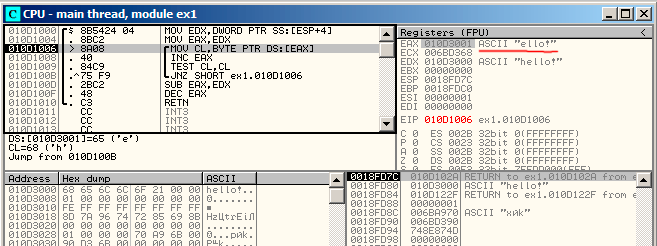
\includegraphics[scale=\FigScale]{patterns/10_strings/1_strlen/olly2.png}
\caption{\olly: \RU{начало второй итерации}\EN{second iteration start}}
\label{fig:strlen_olly_2}
\end{figure}

\RU{Видно, что}\EN{We see that} \EAX \RU{уже содержит адрес второго символа в строке.}
\EN{contains the address of the second character in the string.}

\clearpage
\RU{Будем нажимать F8 достаточное количество раз, чтобы выйти из цикла:}
\EN{We have to press F8 enough number of times in order to escape from the loop:}

\begin{figure}[H]
\centering
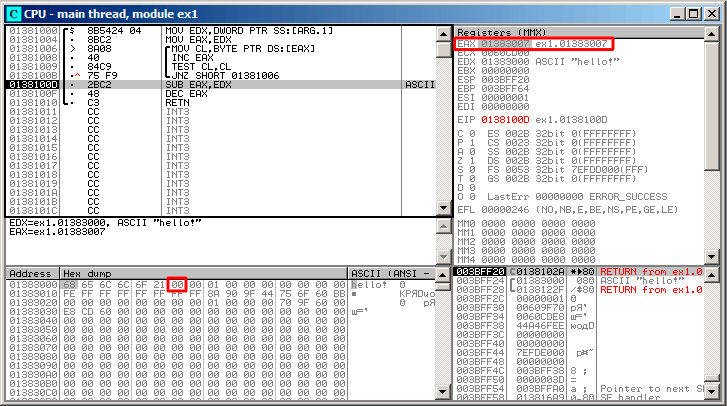
\includegraphics[scale=\FigScale]{patterns/10_strings/1_strlen/olly3.png}
\caption{\olly: \RU{сейчас будет вычисление разницы указателей}\EN{pointers difference to be calculated now}}
\label{fig:strlen_olly_3}
\end{figure}

\RU{Увидим, что \EAX теперь содержит адрес нулевого байта, следующего сразу за строкой.}
\EN{We see that \EAX now contains the address of zero byte that's right after the string.}
\RU{А \EDX так и не менялся~--- он всё ещё указывает на начало строки}\EN{Meanwhile, \EDX hasn't changed,
so it still pointing to the start of the string}.
\RU{Здесь сейчас будет вычисляться разница между этими двумя адресами.}
\EN{The difference between these two addresses is being calculated now.}

\clearpage
\RU{Инструкция \SUB исполнилась}\EN{The \SUB instruction just got executed}:

\begin{figure}[H]
\centering
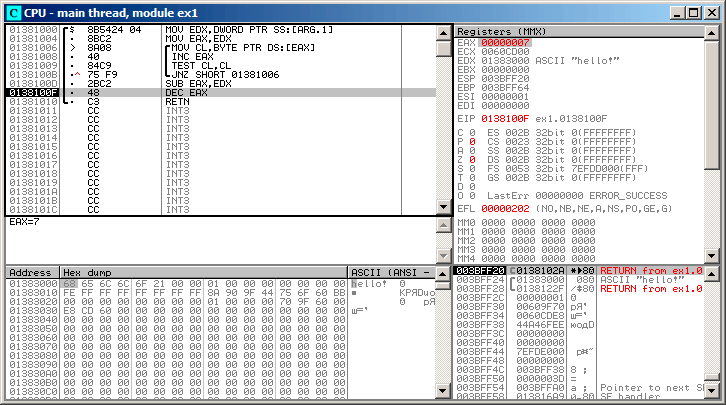
\includegraphics[scale=\FigScale]{patterns/10_strings/1_strlen/olly4.png}
\caption{\olly: \RU{сейчас будет декремент \EAX}\EN{\EAX to be decremented now}}
\label{fig:strlen_olly_4}
\end{figure}

\RU{Разница указателей сейчас в регистре \EAX~--- 7.}
\EN{The difference of pointers is in the \EAX register now---7.}
\RU{Действительно, длина строки}\EN{Indeed, the length of the} \q{hello!}\RU{~--- 6}\EN{ string is 6}, 
\RU{но вместе с нулевым байтом}\EN{but with the zero byte included}\EMDASH{}7.
\RU{Но}\EN{But} \TT{strlen()} 
\RU{должна возвращать количество ненулевых символов в строке.}
\EN{must return the number of non-zero characters in the string.}
\RU{Так что сейчас будет исполняться декремент и выход из функции.}
\EN{So the decrement executes and then the function returns.}
